\documentclass[11pt]{article}

\usepackage{amsmath}
\usepackage{amssymb}
\usepackage{titlesec}
\usepackage[utf8]{inputenc}
\usepackage[margin=2cm]{geometry}
\usepackage{prftree}
\usepackage{changepage}
\usepackage{enumitem}
\usepackage{minted}
\usepackage{graphicx}

\title{\vspace{-2.5cm}CompArch\vspace{-2cm}}
\author{}
\date{}

\setlength{\parindent}{0cm}
\setlength{\parskip}{2mm}
\setlist{nosep}

% Make ~ look more normal
\let\oldsim\sim 
\renewcommand{\sim}{{\oldsim}}

\newminted[monospacefigure]{text}{linenos, frame=lines, framesep=1mm, autogobble, escapeinside=\#\#, mathescape, breaklines, xleftmargin=7mm}

\titlespacing{\section}{0mm}{2mm}{2mm}
\titlespacing{\subsection}{0mm}{2mm}{2mm}
\titlespacing{\subsubsection}{0mm}{2mm}{2mm}

\begin{document}
\maketitle

\section*{Design Metrics}
{ 
    \begin{minipage}[t]{0.3\textwidth}
    \begin{itemize}
    \item Energy
    \item Power
    \item Performance
    \item Security
    \item Cost
    \item Power Efficiency
    \item Reliability
    \end{itemize}
    \end{minipage}
    \begin{minipage}[t]{0.65\textwidth}
    \begin{itemize}
    \item Focus on common case: overall speed increases even if specific speed decreases.
    \item Amdahl's Law: \(\text{speedup} = \frac{1}{\text{sequential} + \frac{1 - \text{sequential}}{\text{speedup}_\text{enhanced}}}\)
    \item Adding enhancements means lower transistor budget, more localised heat, slower clock freq, .... Might affect common case.
    \item
    {
        \[\frac{1}{\text{performance}} = \frac{\text{time}}{\text{program}} = \frac{\text{instructions}}{\text{program}} \times \frac{\text{cycles}}{\text{instruction}} \times \frac{\text{time}}{\text{cycle}}\]

        \begin{itemize}
        \item Instruction count is affected by the ISA and compiler tech.
        \item CPI is affected by micro-architecture and ISA.
        \item Cycle time is affected by circuit design and micro-architecture.
        \end{itemize}
    }
    \end{itemize}
    \end{minipage}
}
\section*{ISAs}
{
    Each ISA is split into the System ISA and the User ISA. System ISA is privileged in some way.

    ISAs either break binary compatibility or carry architectural baggage. Embedded ISAs are more flexible as binary compatibility is less of an issue (mostly purpose-made binaries for product lifetime).

    Can use eg.\ JVM to remove reliance on specific ISA, or allow the processor to dynamically translate (Intel CISC-to-RISC).

    Microcode is code for running the ISA -- miniature control computer. Useful for CISC but introduces performance and complexity overhead.

    RISC ensures instructions are simple for faster fetching, easier pipelining. Relies on compiler to schedule and register-allocate.
}
\section*{Pipelining}
{
    \begin{center}
    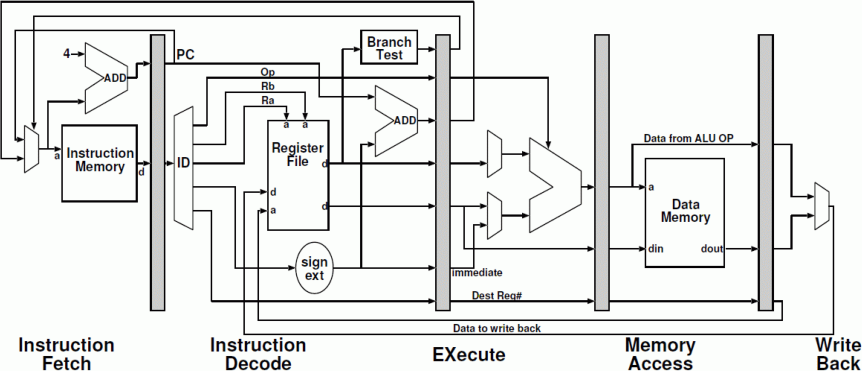
\includegraphics[width=0.8\textwidth]{pipeline.png}
    \end{center}

    \subsection*{Hazards}
    {
        Hazards are phenomena that require stalling in order to preserve program semantics.

        \begin{itemize}
        \item Structural Hazard (CPU resource conflicts, like limited ALU ports)
        \item Data Hazard (inter-instruction dependencies)
        \item Control Hazard (instructions changing the PC like \texttt{jmp})
        \end{itemize}

        \begin{minipage}[t]{0.7\textwidth}
        Instruction dependencies exist between \textbf{any} ordered pairs of instructions, regardless of distance, and make \textbf{reordering} harder.
        \begin{itemize}
        \item
        {
            True data dependence (result is truly required)
            \begin{itemize}
            \item \textbf{RAW}: 1 and 2.
            \end{itemize}
        }
        \item
        {
            Name dependence (same register used for multiple computations)
            \begin{itemize}
            \item \textbf{WAW}: 1 and 4.
            \item \textbf{WAR}: 2 and 3, 2 and 4.
            \end{itemize}
        }
        \end{itemize}
        \end{minipage}
        \begin{minipage}[t]{0.29\textwidth}
        \begin{monospacefigure}
        ADD R1, R2, R3
        SW  R1, 0(R4)
        SUB R4, R3, R5
        ADD R1, R2, R3
        \end{monospacefigure}
        \end{minipage}

        \textit{Structural hazards} can be avoided entirely in hardware/ISA (eg.\ avoid structural by having worst-case number of on-chip resources), but it can slow the common case or simply be too expensive. More complex but faster to handle issues as they come.

        \textit{Data hazards} can be avoided by adding data-forward paths, or scheduling code to prevent data dependencies from becoming data hazards (\textbf{instruction scheduling} by compiler/hardware). Hazards from name dependencies can be solved by \textbf{register renaming} (compiler/hardware).

        \begin{itemize}
        \item Software interlock: compiler inserts instructions on instructions causing a hazard.
        \item Hardware interlock: pipeline stalls when hazards are detected.
        \end{itemize}

        \textit{Control Hazards} can sometimes be avoided by branch prediction. In the simplest pipeline, just stall the fetches until the outcome of the branch is known. For simple tests (\(r = 0\)), could move test and target-address calculation into the decode stage. Requires dedicated hardware and logic for switching to, but reduces the branch delay slot by 1 cycle.
    }
    \subsection*{Exceptions}
    {
        Page fault, illegal op-code, memory protection violation, arithmetic exception, I/O interrupt, ....

        Often want to be able to restart execution after handling the exception: a pipeline supports \textbf{precise exceptions} if it guarantees that all instructions prior to the faulting instruction have been executed and all those after it have not begun execution.

        Simple approach is to tag each instruction with its PC and a flag for whether it raised an exception. Execute stage sets the flag, and stages don't perform side-effects for instructions with the flag set. When the write-back stage sees a faulted instruction it flushes the pipeline.

        Alternatively, hand over control to dedicated hardware when an exception occurs (eg.\ for TLB misses) without flushing the pipeline.
    }
    \subsection*{Multicycle operations}
    {
        Not all instructions can/should complete in a single cycle (eg.\ floating point arithmetic, load/store operations).

        Use multiple execution pipelines, with all the issues arising there: new hazards, harder exception handling, etc.
    }
    \subsection*{Limits}
    {
        \begin{itemize}
        \item Deeper pipelines have more expensive stalls/flushes.
        \item Cycle time determined by worst-case stage time.
        \item Hard to clock each stage at the same time.
        \item More stages increases complexity (forwarding paths, harder exceptions, ...)
        \item Pipelining registers introduce overheads.
        \end{itemize}
    }
    \subsection*{Branch Prediction}
    {
        138g
    }
}
\end{document}